% !TEX root = robobrain.tex
\section{System Architecture}
\label{sec:system}
\begin{figure}[t]
\centering
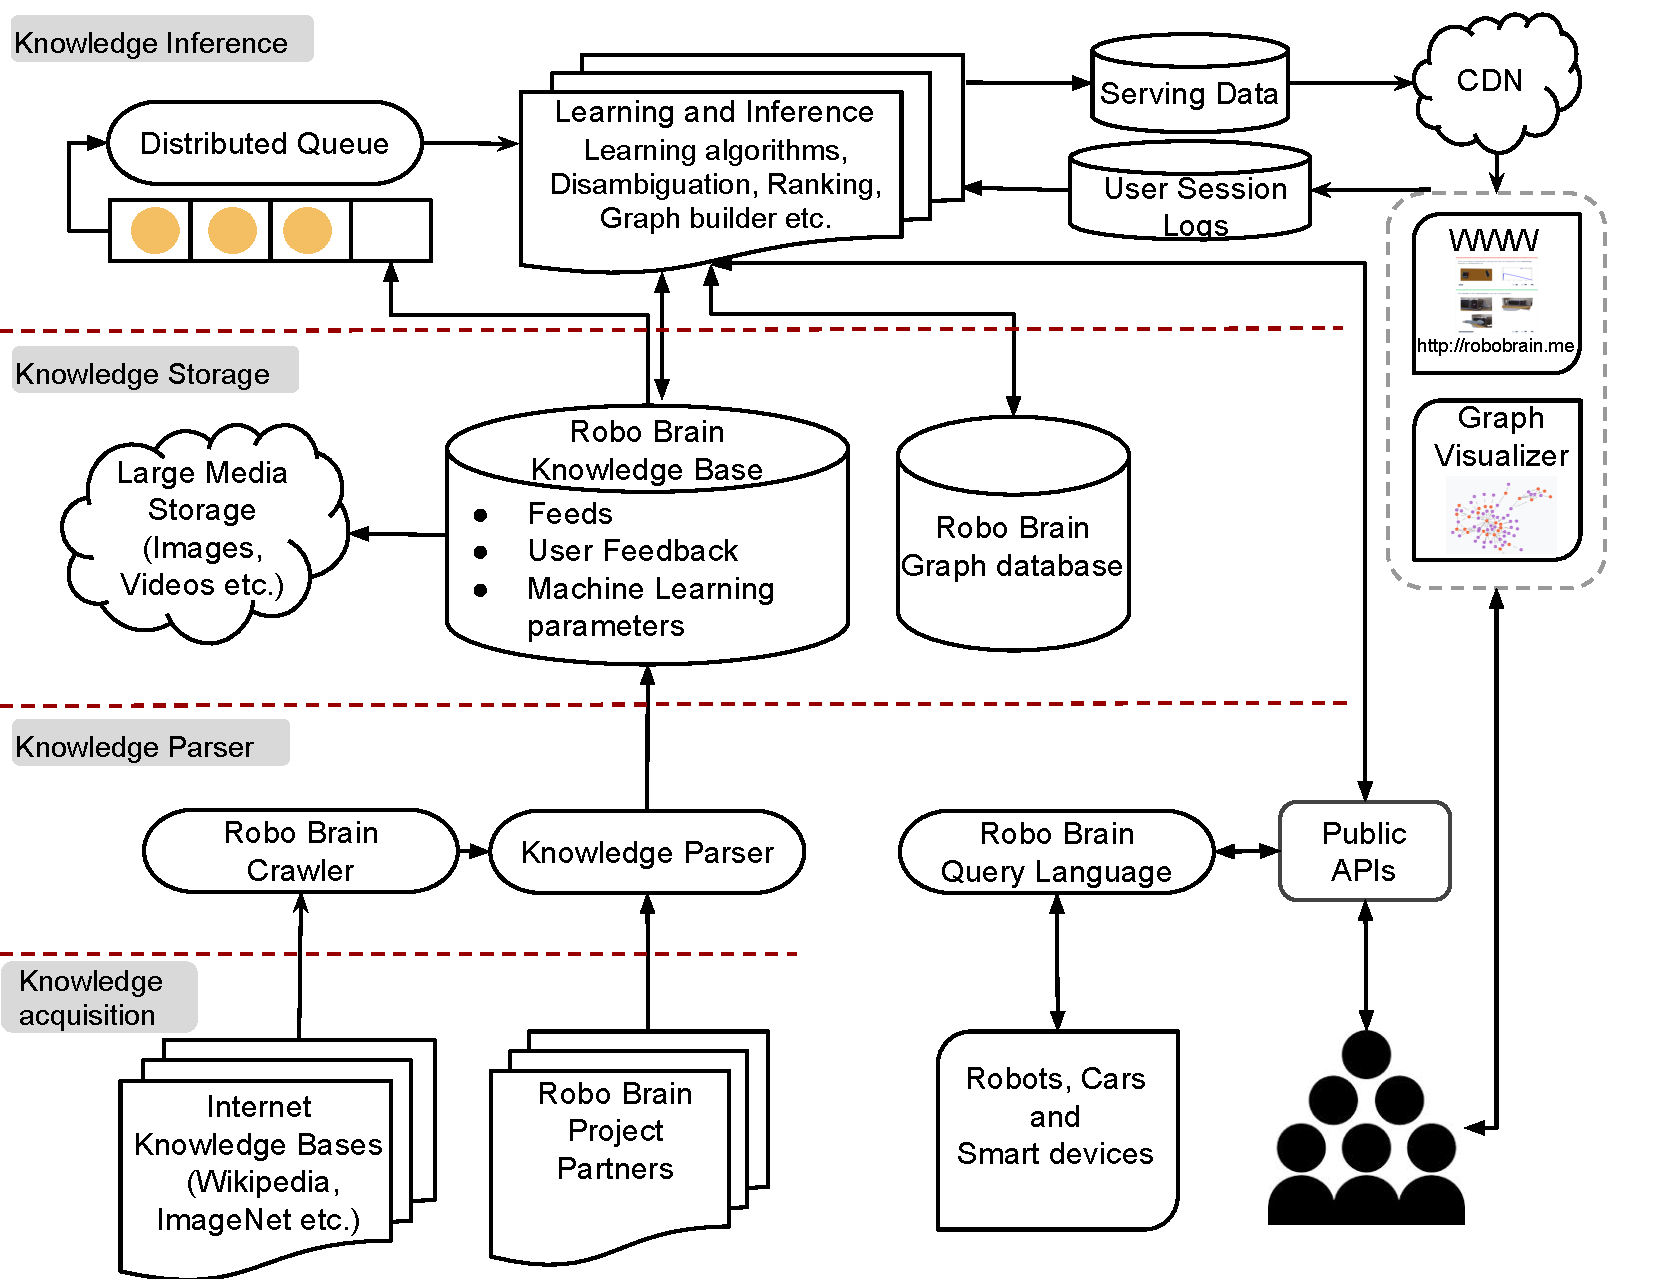
\includegraphics[width=\linewidth]{Image/RoboBrain_Systems}
\caption{\textbf{\robobrain{} system architecture.} It consists of four
interconnected knowledge layers and supports various mechanisms for users and
robots to interact with \robobrain{}.}
\label{fig:system}
\end{figure}

% \todo {This is just a first pass to set the basic coverage of the section}

We now describe the system architecture of \robobrain{}, shown in Figure~\ref{fig:system}. The system
consists of four interconnected layers: (a) knowledge acquisition, (b) knowledge
parser, (c) knowledge storage,  and (d) knowledge inference. The principle
behind our design is to efficiently process large amount of unstructured
multi-modal knowledge and represent it using the structured \mbox{\robobrain{}} graph.
In addition, our design also supports various mechanisms for users and robots to interact with \robobrain{}. %Through these interactions users retrieve knowledge and also improve \robobrain{} through feedback. 
Below we discuss each of the components.
%and (e) interaction mechanisms.

% It also comprises interactions with robots and users via physical and online interactions.

% many layers and most of the components are restful (Need to write more).

\textit{Knowledge acquisition} layer is the interface between \robobrain{} and the
different sources of multi-modal data. Through this layer \robobrain{} gets access to new information which the other layers process.  \robobrain{} primarily collects knowledge through its partner projects and by crawling the existing knowledge bases such as Freebase, ImageNet and WordNet, etc.,  as well as unstructured sources such as  Wikipedia.


\textit{Knowledge parser} layer of \robobrain{} processes the data acquired by the acquisition layer and converts it to a consistent format for the storage layer. It also marks the incoming data with appropriate meta- data such as  timestamps, source version number etc., for scheduling and managing future data processing. Moreover, since the knowledge bases might change with time, it adds a back pointer to the original source.

\textit{Knowledge storage} layer of \robobrain{} is responsible for storing different representations of the data. In particular it consists of a NoSQL document storage database cluster -- \robobrain{} Knowledge Base (\robobrain{}-KB) -- to store ``feeds'' parsed by the knowledge parser, crowd-sourcing feedback from users, and parameters of different machine learning algorithms provided by \robobrain{} project partners. \robobrain{}-KB offloads large media content such as images, videos and 3D point clouds to a distributed object storage system built using Amazon Simple Storage Service (S3). The real power of \robobrain{} comes through its graph database (\robobrain{}-GD) which stores the structured knowledge. The data from \robobrain{}-KB is refined through multiple learning algorithms and its graph representation is stored in \robobrain{}-GD. The purpose behind this design is to keep \robobrain{}-KB as the \robobrain{}'s single source of truth (SSOT). SSOT centric design allows us to re-build \robobrain{}-GD in case of failures or malicious knowledge sources.

\textit{Knowledge inference} layer contains the key processing and machine learning components of \robobrain{}. All the new and recently updated feeds go through a persistent replicated distributed queuing system (Amazon SQS), which are then consumed by some of our machine learning plugins (inference algorithm, graph builder, etc.) and populates the graph database. These plugins along with  other learning algorithms (operating on the entire graph) constitute our learning and inference framework. 

\robobrain{} supports various \textit{interaction mechanisms} to enable robots and users to communicate with the knowledge engine.
We develop a Robot Query Library as a primary method for robots to interact with \robobrain{}. We also make available a set of public APIs to allow information to be presented on the WWW for online learning mechanisms (eg., crowd-sourcing). \robobrain{} serves all its data using a commercial content delivery network (CDN) to reduce the end user latency. 